\documentclass[11pt]{report}
\usepackage[utf8]{inputenc}
\usepackage{graphicx}
\usepackage{amsmath}
\usepackage[T1]{fontenc}
\usepackage{babel}
\usepackage{lipsum}
\usepackage{subfigure}
\usepackage{gensymb}
\usepackage[normalem]{ulem}
\useunder{\uline}{\ul}{}
\usepackage[table,xcdraw]{xcolor}
\usepackage[font=small,labelfont=bf,textfont=it]{caption} %pacchetto per modificare il caption delle immagini
 
\title{Wireless Electromagnetic Technologies\newline\begin{small}(ICT and Internet Engineering - 9 CFU)\end{small}}

\author{
  Fallani Rebecca\\
  \texttt{rebeccafallani23@gmail.com}
  \and
  Riolo Ivan\\
  \texttt{ivan.riolo@hotmail.it}
   \and
  Savini Davide\\
  \texttt{davide.savini95@gmail.com}
}
\date{January 2021}

\begin{document}
\maketitle
\thispagestyle{empty}
\tableofcontents
\thispagestyle{empty}
\chapter*{Introduction}
\addcontentsline{toc}{chapter}{Introduction}
\thispagestyle{empty}
\markboth{INTRODUCTION}{}

The project is divided into three main points, respectively A,B and C, follow a briefly description. The design process was performed on Matlab with Antenna Toolbox and its following apps: Antenna Designer, PCB Antenna Designer and Sensor Array Analyzer.
\section*{A - Tchebyshev array synthesis}
The first point requires the design of an array using Tchebyshev's synthesis procedure. The number of elements to be used is 5 and the main lobe/secondary lobe ratio to satisfy is 120 (linear).
\section*{B - Folded patch}
The second point requires the design of a rectangular folded patch fed by coaxial cable, whose dimensions must be compatible with the parameters of the array designed in the previous point.
\section*{C - Overall array}
The last point requires evaluating the performance of the overall designed array in which the single element is the folded patch designed in the point B, both in broadside pointing and rotated of 45 degrees from the boresight direction pointing.
\newpage
% diagramma di flusso
\thispagestyle{empty}
\begin{figure}[h!]
    \centering
    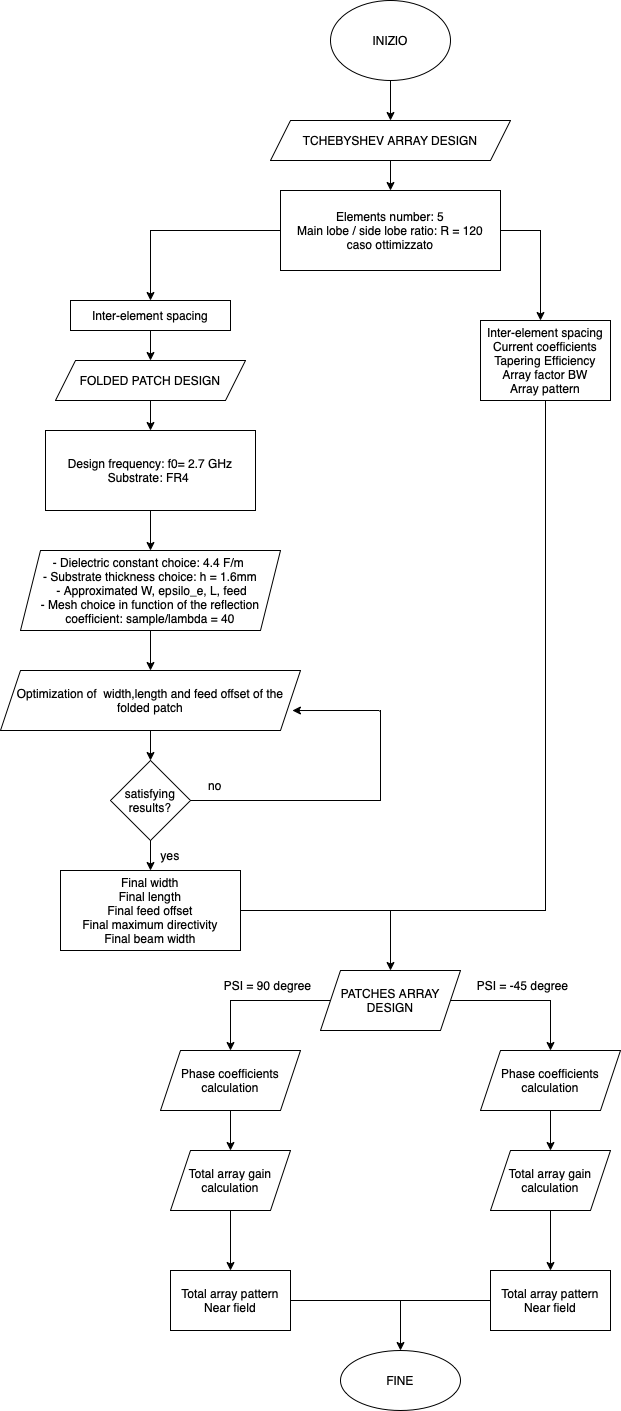
\includegraphics[width=9cm]{Pictures/Diagram.drawio-2.png}
    \textit{\caption{Flow chart of the whole design process}}
\end{figure}

\setcounter{page}{0}
\chapter{Tchebyshev array synthesis}
The Tchebyshev synthesis procedure is shown in the case of inter-elements spacing $ \lambda/2<d<\lambda $ (optimised case), in order to achieve the fixed Main Lobe Side Lobe ratio specified R = 120 (linear) with a number of elements M = 5:

\begin{equation}
\left|\frac{F(M L)}{F\left(S L_{\max }\right)}\right|=R
\end{equation}

\begin{equation}
M = 2N + 1 = 5.
\end{equation}
So, it is possible to determine N equal to 2 as the degree of requested Tchebyshev polynomial for the synthesis. The first thing to do is to determine the visibility window in Tchebyshev's domain, considering the unitary cage in order to limit the SL within it. Then it is extended to  $x_{1}$ in order to choose the ML with the desired R, so we have $ -1<VW(x)<x_{1} $. \newline
At this point we know all the information necessary to determine $x_{1}$:

\begin{equation}
x_{1}=\cosh \left(\frac{1}{N} \cosh ^{-1} R\right)=7.78.
\end{equation}

From the mapping between the domain of Tchebyshev ($x$) and the domain of the transition variable ($u$), given by $ x = a + b cos(u) $, we can determine the parameters $a$ and $b$ and the the value of $k_{0}d$ as follow.

\begin{equation}
\left\{\begin{array}{l}
a=\frac{x_{1}-1}{2} \\
b=\frac{x_{1}+1}{2}\\
a + b\cos{k_{0}d} = 1
\end{array}\right.
\end{equation} 

The solutions are:

\begin{equation}
\left\{\begin{array}{l}
a=3,39 \\
b=4,39\\
k_{0}d = \{ \frac{41}{60}\pi \ ; \frac{79}{60}\pi\}
\end{array}\right.
\end{equation} 

In order to optimize, we choose the maximum $k_{0}d$ that satisfy $ \lambda/2<d<\lambda $ that means $ \pi<k_{0}d<2\pi $. The value $\frac{79}{60}\pi$ that is equal to $ 237\degree$ meets this condition . Consequently we obtain an inter-distance value in function of lambda equal to:

\begin{equation}
d = \frac{79}{120}\lambda.
\end{equation}

From Tchebyshev polynomial of order $N=2$ it possible to calculate the current coefficients $C_{n}$, knowing the parameters $a$ and $b$. (Paying attention to coefficients greater than the first, which must be divided by 2).

\begin{equation}
T_{2}(a+b \cos (u))=\left(2 a^{2}+b^{2}-1\right)+4 a b \cos (u)+b^{2} \cos (2 u).
\end{equation}
So we have:
\begin{equation}
C_{0}=2 a^{2}+b^{2}-1=41.26 ; \quad C_{1}=2 a b=29.76 ; \quad C_{2}=\frac{b^{2}}{2}=9.64.
\end{equation}

It's possible to evaluate also the ratio between the maximum and minimum $C_{n}$ as follow:

\begin{equation}
\frac{C_{max}}{C_{min}}=4.28.
\end{equation}

It's important to evaluate the tapering efficiency due to the non uniform feed, that is:
\begin{equation}
\eta_{T}=\frac{1}{2 N+1}\left(\frac{\left|\sum\right| C_{n}||^{2}}{\sum|C n|^{2}}\right)=\frac{1}{5}\left(\frac{\left|C_{0}+2 C_{1}+2 C_{2}\right|^{2}}{C_{0}^{2}+2 C_{1}^{2}+2 C_{2}^{2}}\right)=78 \%.
\end{equation}

In order to evaluate the FNBW, is possible to calculate the first null $x_{0}$ in Tchebyshev domain, then report it in the $u_{0}$ domain and in the end we obtain $\phi_{0} $ that is the angle to the first null in the polar diagram. The passages are reported below.

\begin{equation}
\quad x_{0}=\cos \left(\frac{(2l-1)\pi}{2N}\right);
\quad u_{0}=\cos ^{-1}\left(\frac{x_{0}-a}{b}\right); 
\quad \psi_{0}=\cos ^{-1}\left(\frac{u_{0}}{k_{0} d}\right).
\end{equation}

Where $\frac{(2l-1)\pi}{2N}$ evaluated for $l=1$ is the first zero. The next zeros are derived for $l=2,3,4$. The formula is obtained exploiting the property of Tchebyshev polynomial $T_{N}(cos(x))=0$ is equal to $cos(Nx)=0$.  The results are: $x_{0} = 0.7071$, $u_{0} = 127\degree$ and $\phi_{0} = 58\degree$. So the First Null Beamwidth is:
\begin{equation}
FNBW = \pi - 2\phi_{0} = 65.3\degree.
\end{equation}
The FNBW of an array of the same size but uniformly fed is:
\begin{equation}
B W=\frac{2 \lambda}{(N+1) d} = 34.83\degree.
\end{equation}
As can be seen, the price to pay for a better ML/SL ratio is a much wider FNBW (almost twice the FNBW of uniform case) and a reduced tapering efficiency. The feed coefficients, the rectangular and polar diagrams are shown below.

\begin{figure} [h!]
\begin{minipage}[b]{7cm}
\centering
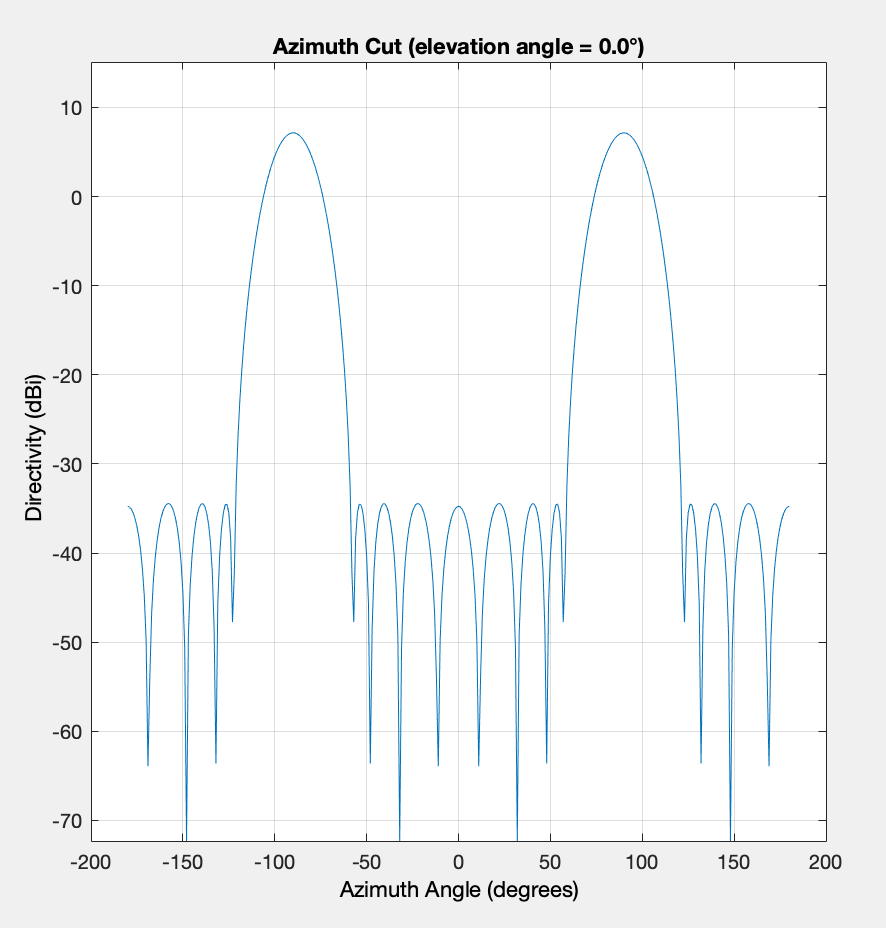
\includegraphics[width=6.5cm]{Pictures/rectangular_diagram.png}
\textit{\caption{Rectangular diagram}}
\label{Tchebyshev_pl}
\end{minipage}
\ \hspace{2mm} \hspace{3mm} \
\begin{minipage}[b]{7cm}
\centering
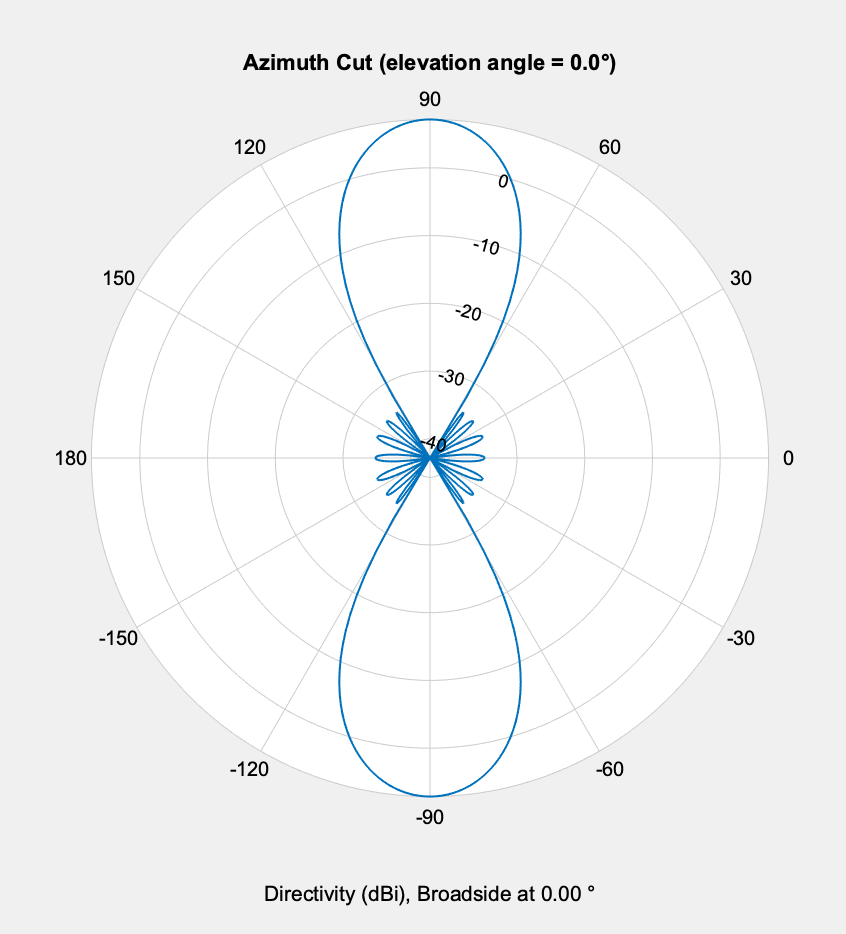
\includegraphics[width=6.5cm]{Pictures/polar_diagram.png}
\textit{\caption{Polar diagram}}
\end{minipage}
\end{figure}

It's possible to see in the figure 1.2, there are three and a half side lobes, as there are 2 zeros of the Tchebyshev polynomial and they are each mapped to 4 zeros of the u-space, giving a total of 8 zeros in u-sapce.

\chapter{Folded patch}
\section{Starting design}
The project specifications requires a rectangular folded patch fed by a coaxial cable at frequency of 2.7 GHz, whose size is compatible with the inter-antenna distance derived in Tchebyshev synthesis.\newline
The FR4 substrate is mandatory for the design, it is suitable for miniaturized antennas thanks to high $\epsilon_{r}$ values that permit to achieve length in the order of mm. It has also good resistance to high temperature and a considerable mechanical strength. It's also a low cost material.\newline The first step is to choice the thickness $h$ among the possible solutions: ${0.8 ~mm, 1.0 ~mm , 1.6 ~mm}$.  The choice falls on:

\begin{equation}
h=1.6 \mathrm{~mm} \quad with \quad \varepsilon_{r}=4.4.
\end{equation}

This choice is made in order to decrease the Quality Factor, so to increase the Bandwidth. Considering that the folded patch has a very low bandwidth values in term of fractional bandwidth, around $0.5\% - 1\%$. As can be seen from the following relationships:
\begin{equation}
\begin{array}{l}
Q_{T} \propto \frac{\varepsilon_{r}}{h+\varepsilon_{r} \cdot \tan (\delta)} \quad \text{and} \quad
B \propto \frac{1}{Q_{T}}
\end{array}
\end{equation}
follow that to increase B we have to choose an higher h.\newline Then the value of dielectric constant suitable for the operating frequency (2.7 GHz) is determined following a constructor and literature search. It shows that FR4's $\epsilon_{r}$ vary from vendor, thickness and percentage of epoxy resin.
Many studies (e.g studies done by Rogers) performs some measurements on $\epsilon_{r}$ by means of a resonant circuit called O-Ring and confirm the choice made.


%The choice of the relative dielectric constant was made by carrying out a cross study of two measurements made by Rogers on dielectrics through the resonance circuit called the Resonator Ring (O-ring). The circuit works in a frequency range of 2-10 GHz and its structure allows for: no Fringe Effect, no spurious modes, negligible radiation losses. \newline
%This clarification allows approximations with minimal errors to the measurement. The measurement takes place with the circuit resonating at different frequencies; the relative dielectric constant is measured in the resonance peaks. At frequencies around 2.7 GHz the relative dielectric constant has values ranging between 4.3 and 4.5 and therefore the average value 4.4 was chosen.
Now is possible to compute the first approximated dimensions of folded patch by means of the Balanis formulas (it's important to note that some variations to the formulas are necessary because they refer to the classic $\lambda/2$ patch). At the operating frequency of 2.7 GHz, we have:
\begin{equation}
\lambda_{0}=\frac{c_{0}}{f_{0}}=0.111 \mathrm{~m} \text{, } \quad k_{0}=\frac{2 \pi}{\lambda_{0}}=56.5878 \mathrm{~m}^{-1}.
\end{equation}

The thickness $h$ is checked with respect to $h_{\max}$ verifying the relationship: $h \leq h_{\max }$  with $h_{\max }=\frac{0.3 \lambda_{0}}{2 \pi \sqrt{\epsilon_{r}}}=2.7 \mathrm{~mm}$ 
\begin{equation}
W=\frac{c_{0}}{2 f_{0}} \sqrt{\frac{2}{\epsilon_{r}+1}}=33.8 \mathrm{~mm}.
\end{equation}
With the following relationships
$$
\begin{array}{l}
\epsilon_{\mathrm{eff}}=\frac{\epsilon_{r}+1}{2}+\frac{\epsilon_{r}-1}{2}\left(1+12 \frac{h}{W}\right)^{-\frac{1}{2}} \text { and } \Delta L=0.412 h \frac{\left(\epsilon_{\mathrm{eff}}+0.3\right)\left(\frac{W}{h}+0.264\right)}{\left(\epsilon_{\mathrm{eff}}-0.258\right)\left(\frac{W}{h}+0.8\right)} \\
\end{array}
$$
we can find:
\begin{equation}
L=L_{e f f}- \Delta L=\frac{c_{0}}{4 f_{0} \sqrt{\epsilon_{e f f}}}- \Delta L=13 \mathrm{~mm}.
\end{equation}
The effective length is now equal to $\frac{\lambda}{4}$ in order to achieve the miniaturization. While the radiation resistance, by considering the slot model that represents the patch, we have only one radiating slot instead of two, follow that radiation resistance is the double of a regular patch ($\frac{\lambda}{2}$):
\begin{equation}
R_{r}=\frac{1}{G_{s}}=\frac{120 \lambda_{0}}{W}\left(1-\frac{1}{24}\left(k_{0} h\right)^{2}\right)^{-1}=394.5 ~\Omega.
\end{equation}
In order to adapt the input resistance to $R_{i n}=50 \Omega$ the feed port is moved by $l$ (from radiating side):
\begin{equation}
l=\frac{1}{\beta} \operatorname{acos} \sqrt{\frac{R_{i n}}{R_{r}}}=10 \mathrm{~mm}
\end{equation}
with $\beta=\frac{2 \pi}{\lambda_{0}} \sqrt{\epsilon_{r}}$ approximated to $\beta=\frac{\pi}{2L}.$ It's possible to note that, having a double radiation resistance respect to $\frac{\lambda}{2}$ patch, it is necessary to move the feed more towards the short circuit.
\newline

To compute the directivity we consider the classic patch formula that come from the two-slot radiant model and we consider that for the folded patch directivity is approximately the half of it:
\begin{equation}
D_{0}=\frac{2}{15}\left(\frac{W}{\lambda_{0}}\right)^{2} R_{r}=5.0601\implies D\cong\frac{D_{0}}{2}=2.5301.
\end{equation}

In order to compute the beamwidth for the folded patch is possible to consider the single radiant slot model in order to have an analytical visualization. In the E-cut $\theta = \pi/2$ the far field of a slot not depend by azimuth angle, so we have a constant radiation pattern and consequently the $BW_{e}$ is 180$\degree$. Using Matlab to measure the beamwidth, this theoretical discussion is confirmed.
For the beamwidth on the H-cut the radiation pattern of single radiant slot depend on $\theta$ in the same way of double radiant slot model. So it's possible to use the formula for the $\lambda/2$ patch:
\begin{equation}
\mathrm{BW}_{h}=2 \operatorname{acos}\left(\sqrt{\frac{1}{2+k_{0} W}}\right)=119\degree.
\end{equation}

%beamwidth figure

\begin{figure} [h!]
\begin{minipage}[b]{6.8cm}
\centering
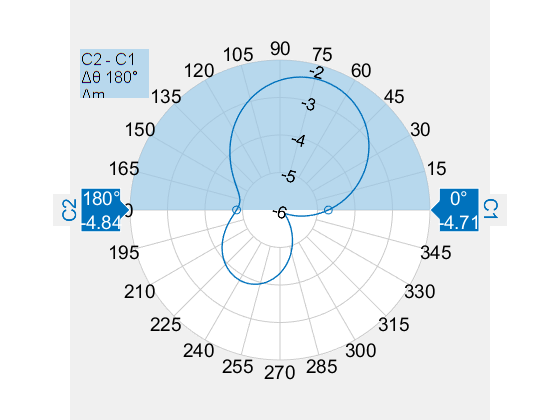
\includegraphics[width=7cm]{Pictures/beamwidth_chapter_2/BW_E_cut_starting.png}
\textit{\caption{E-cut of starting patch}}
\end{minipage}
\ \hspace{2mm} \hspace{3mm} \
\begin{minipage}[b]{6.8cm}
\centering
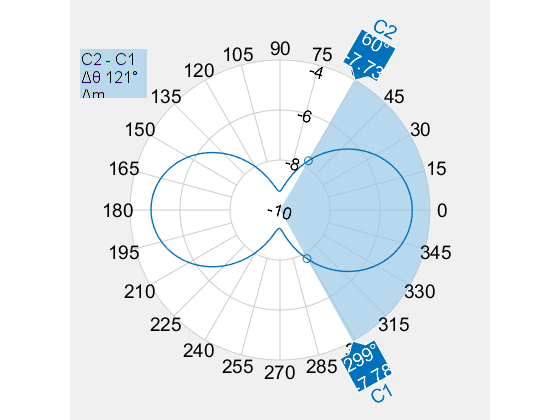
\includegraphics[width=7cm]{Pictures/beamwidth_chapter_2/BW_H_cut_starting_pifa.png}
\textit{\caption{H-cut of starting patch}}
\end{minipage}
\end{figure}

\newpage
\section{Mesh choice and optimization}
It's important to choose the correct mesh parameter before carrying out the optimization, in order to have reliable results. Starting from the approximated prototype, the reflection coefficient was evaluated from 2 GHz to 3.3 GHz with 14 intermediate frequencies for 90 different mesh configurations. For each one the frequency of minimum $\Gamma$ is saved. In figure 2.3 the result is shown.

\begin{figure}[h!]
    \centering
    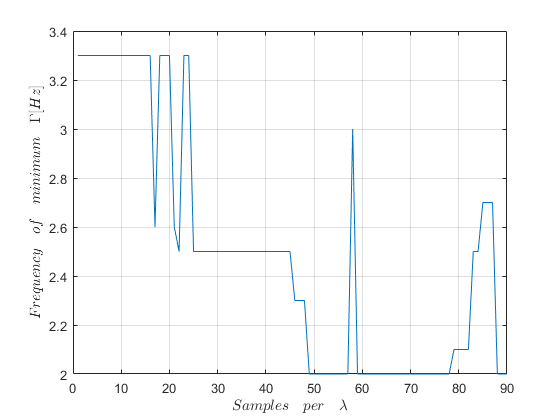
\includegraphics[width=10cm]{Pictures/pifa_mesh_ultima.png}
    \textit{\caption{Frequency corresponding to the minimum of the reflection coefficient as a function of the samples per $\lambda$.}}
    \label{mesh}
\end{figure}

It can be deduced that for values between 25 and 45 of samples per lambda there is the constant region of resonant frequency. The most efficient choice of mesh to avoid long calculation times and have reliable results is $\lambda/30$. In order to desing and visualize the starting antenna the Matlab tool Antenna Designer is used. Then optimization is performed by varying the geometric parameters W and L in order to obtain the resonance at the operating frequency $2.7 \mathrm{~GHz}$ and to minimize the reflection coefficient. Once the tests were performed, the optimal parameter chosen, which determines a reflection coefficient of about $-39.8 ~dB$, are the follow:
\begin{equation}
W=37.1 \mathrm{~mm,} \quad L=12.1 \mathrm{~mm}.
\end{equation}

% contour
%Through Antenna Toolbox, for each optimization, intermediate files are generated before reaching the final optimization; within these files, there are the values of w and L and the relative gamma value. Once this set of values has been obtained, they are collected in the two-dimensional graph in figure 2.2 to visualize the range trend at various of w and L until the optimized case in figure 2.3 is reached.
We start with a coarse vary of L and W, L $\pm ~3 ~mm$ and W $\pm ~3.8 ~mm$, in order to find L values that shift the resonance precisely to 2.7 GHz (the resonance depend strictly on the lenght). For each combination of L and W the measure of $\Gamma$ at center frequency is perfomed. As can be seen in figure 2.4 obtained with contour Matlab function, the range of interest of L and W are retrieved. Then focusing on $11.8<L<12.4 ~mm$ and $ 35<W<37.6 ~mm$, a second cycle of measurements are performed and the result are shown in figure 2.5. The results are optimal values of $L = 0.0122 ~mm \text{ and } W = 0.0375 ~mm$, that give us a $\Gamma = -39.8dB$. To obtain more realistic results and overcome many problem of Antenna toolbox (feed too near the short circuit) we moved the optimized PIFA object to PCB toolbox by recreating the short circuit with the use of 9 vias. 
By positioning the vias at the correct distance the short circuit is obtained, in order to achieve a better result a final manual variation is performed on L, W and feed point of $\pm ~0.1 ~mm$. The final result is $\Gamma = -40~dB $ with $L = 0.0121 ~m, W  = 0.0371 ~m \text{ and feed at } 2.5 ~mm$ from short circuit.


\begin{figure} [h!]
\begin{minipage}[b]{7.5cm}
\centering
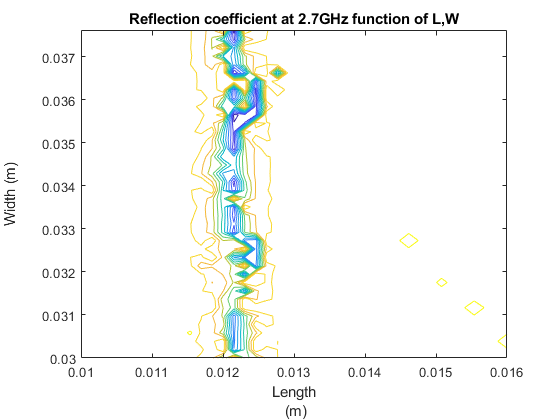
\includegraphics[width=7cm]{Pictures/contour_figure.png}
\textit{\caption{Two-dimensional representation of $~\Gamma $ as a function of w and L - non-optimized case}}
\end{minipage}
\ \hspace{2mm} \hspace{3mm} \
\begin{minipage}[b]{7.5cm}
\centering
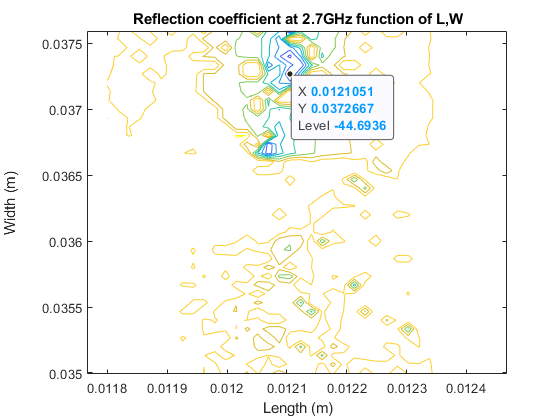
\includegraphics[width=7cm]{Pictures/contour_refine.png}
\textit{\caption{Two-dimensional representation of $~\Gamma $ as a function of w and L - optimized case}}
\end{minipage}
\end{figure}

\section{Performance analysis after optimizations}
Having found the optimal geometry for our patch, we move on to the representation of the performance; follow the set of graph that represents the fundamental parameters of the antenna. 
\begin{figure} [h!]
\begin{minipage}[b]{7.5cm}
\centering
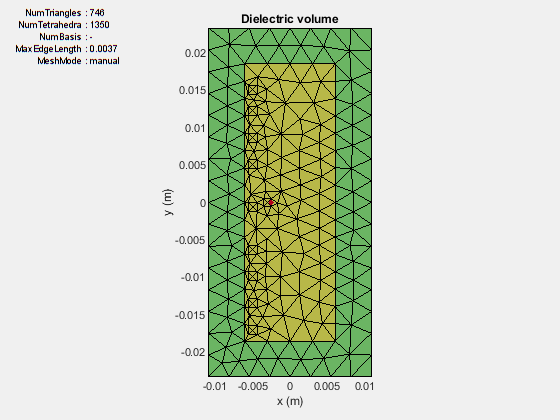
\includegraphics[width=7.5cm]{Pictures/grafici_prestazionali/mesh pcb su xy.png}
\textit{\caption{PCB mesh on xy plane}}
\end{minipage}
\ \hspace{2mm} \hspace{3mm} \
\begin{minipage}[b]{7.5cm}
\centering
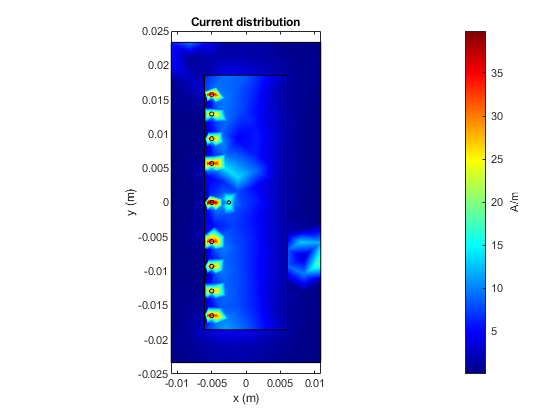
\includegraphics[width=7.5cm]{Pictures/grafici_prestazionali/correnti su xy.png}
\textit{\caption{Current phasor value on xy plane}}
\end{minipage}
\end{figure}

Figure 2.6 show the PCB mesh of our patch while figure 2.7 shows the orientation of the currents on the xy plane.
In the following figures we appreciate the images of: input impedance with input reactance, reflection coefficient, radiation pattern and gain pattern on H-cut and E-cut.

\begin{figure} [h!]
\begin{minipage}[b]{7cm}
\centering
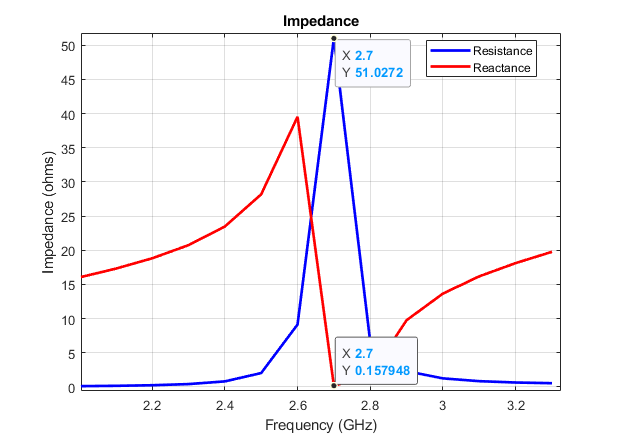
\includegraphics[width=8cm]{Pictures/grafici_prestazionali/impedenza_e_reattanza_finale.png}
\textit{\caption{Input impedance and input reactance}}
\end{minipage}
\ \hspace{2mm} \hspace{3mm} \
\begin{minipage}[b]{7cm}
\centering
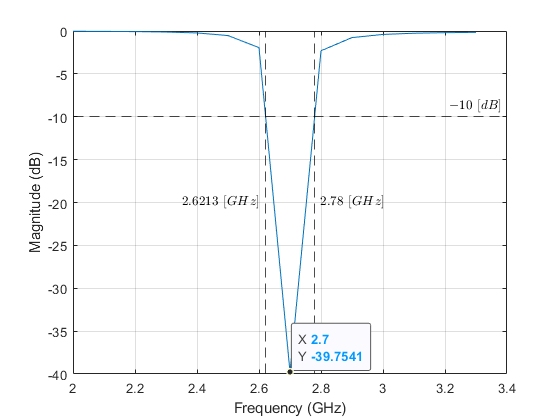
\includegraphics[width=8cm]{Pictures/grafici_prestazionali/sparameter_con_valori_s11_optimized_con_Banda_new_new.png}
\textit{\caption{Reflection coefficient on the operating frequency}}
\end{minipage}
\end{figure}

As can be seen from figure 2.8, at the working frequency 2.7 GHz, there is an input impedance around 50 $\ohm$ and an input reactance close to zero. In figure 2.9, at the operating frequency and bandwidth at $-10 ~dB$ equal to 158.7 MHz, a good reflection coefficient is observed at $-39.7541 ~dB$. The following images shows the radiation diagrams in order to be able to observe the gain of our optimized antenna patch. 

\begin{figure}[h!]
    \centering
    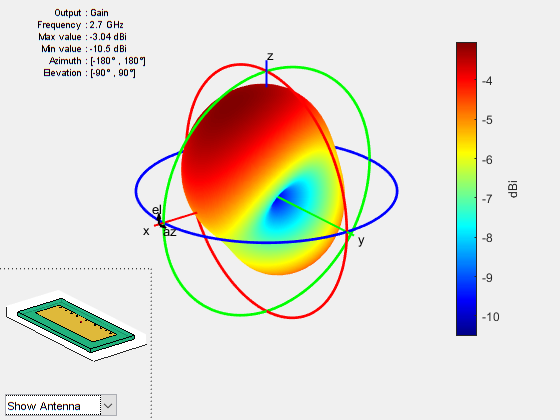
\includegraphics[width=8cm]{Pictures/grafici_prestazionali/pattern.png}
    \textit{\caption{Radiation pattern; visible patch on lower left side}}
    \label{3D_pattern}
\end{figure}

\newpage
Figure 2.10 shows the radiation pattern with the visible patch.
Figure 2.11 shows the radiation pattern on H-cut and figure 2.12 represents the radiation pattern on E-cut with the obtained Gain on 2.7 GHz equal to $-3.04 ~dBi$.

\begin{figure} [h!]
\begin{minipage}[b]{6.8cm}
\centering
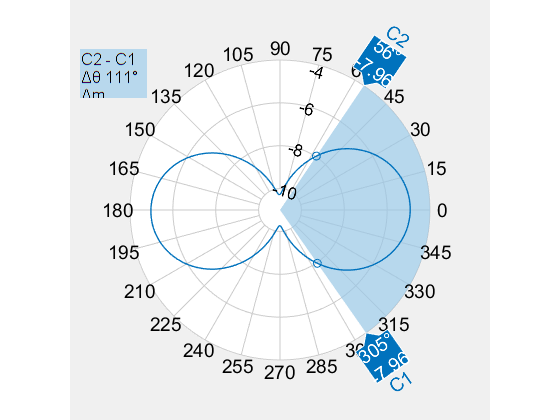
\includegraphics[width=8cm]{Pictures/beamwidth_chapter_2/BW_H_cut_final.png}
\textit{\caption{BW on H-cut of final patch}}
\end{minipage}
\ \hspace{2mm} \hspace{3mm} \
\begin{minipage}[b]{6.8cm}
\centering
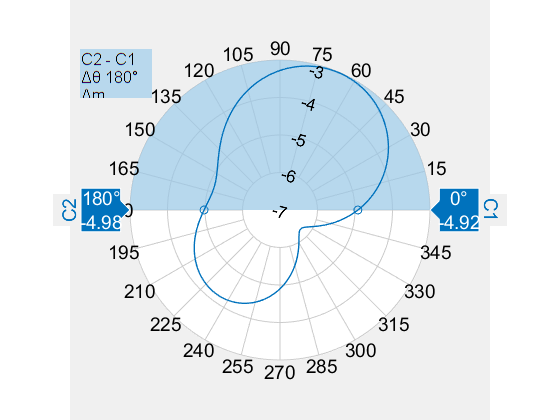
\includegraphics[width=8cm]{Pictures/beamwidth_chapter_2/BW_E_cut_final.png}
\textit{\caption{BW on E-cut of final patch}}
\end{minipage}
\end{figure}

\newpage %se tolto, quanto scritto, va una pagina indietro
We can appreciate a recap of the main characteristic parameters of the optimized patch in the following table:
\begin{table}[h!]
\textit{\caption{Parameter comparison between initial patch and optimized patch}}
\centering
\medskip
\begin{tabular}{lll}
\hline
Characteristic parameters & Optimized Patch \\ \hline
$|Z_{in}|$                &       51.0272 $\ohm$       \\
$R_{in}$                  &       51.0272 $\ohm$       \\
$X_{in}$                  &       0.1579 $\ohm$        \\
$|\Gamma_{f_{0}}|_{dB}$   &       -39.754 $dB$         \\
$B_{-10dB}$               &       158.7 $MHz$          \\
$G_{max,dBi}$             &       -3.04 $dBi$          \\
$BW_{-3dB,zx}$            &       180$\degree$         \\
$BW_{-3dB,zy}$            &       111$\degree$         \\ \hline
\end{tabular}
\end{table}

\chapter{Overall array}
\section{Phase shift}
In order to compute the phase coefficients the following formula is used.
\begin{equation}
k_{0} d \cos \varphi_{0}=-\alpha d
\end{equation}
The broadside steering is characterized from a null phase shifting, so all the phase coefficients are set to the same value $\alpha = 0\quad then\quad \phi_{0}=0$.
The following table shows the phase values for each radiating element in order to achieve the beamsteering of 45 $\degree$ off the boreshight.
\begin{table}[h!]
\textit{\caption{Phase coefficients}}
\centering
\medskip
\begin{tabular}{|
>{\columncolor[HTML]{FFFFFF}}l |
>{\columncolor[HTML]{FFFFFF}}l |
>{\columncolor[HTML]{FFFFFF}}l |
>{\columncolor[HTML]{FFFFFF}}l |
>{\columncolor[HTML]{FFFFFF}}l |
>{\columncolor[HTML]{FFFFFF}}l |}
\hline
{\color[HTML]{000000} \textbf{Position element (n)}} & {\color[HTML]{000000} \textbf{0}} & {\color[HTML]{000000} \textbf{1}}  & \textbf{2} & \textbf{3} & \textbf{4} \\ \hline
{\color[HTML]{000000} $n\cdot u_{0}$}                       & {\color[HTML]{000000} 0 rad}   & {\color[HTML]{000000} 2.925 rad}  & 5.85 rad      & 8.775 rad  & 11.7 rad   \\ \hline
\end{tabular}
\label{tab:phase coefficients}
\end{table}

%PATTERN ARRAY UNIFORME
In the following figures we have the uniform array pattern with its Azimuth-cut and its rectangular pattern. 

\begin{figure}[!htb]
\minipage{0.322\textwidth}
  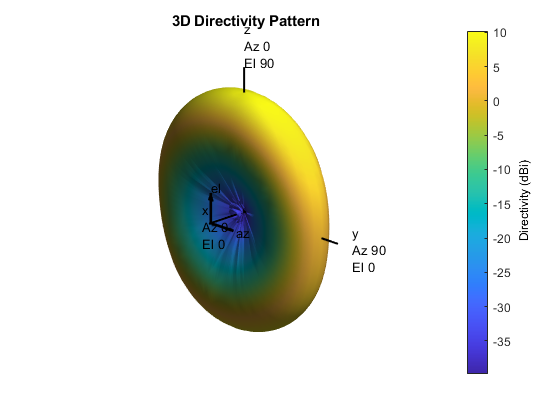
\includegraphics[width=\linewidth]{Pictures/overall_array/3Dpattern.png}
  \textit{\caption{Radiation pattern}\label{fig:immagine01}}
\endminipage\hfill
\minipage{0.322\textwidth}
  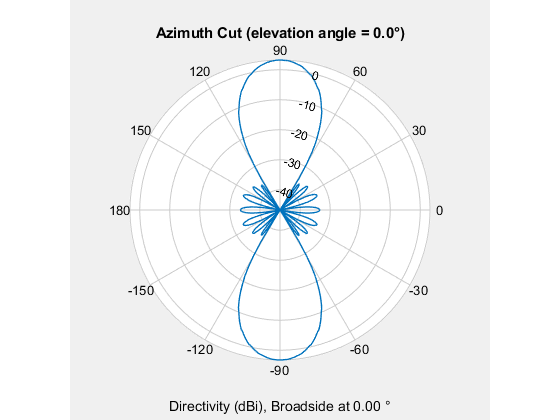
\includegraphics[width=\linewidth]{Pictures/overall_array/azimuth.png}
  \textit{\caption{Azimuth-cut}\label{fig:immagine2}}
\endminipage\hfill
\minipage{0.322\textwidth}
  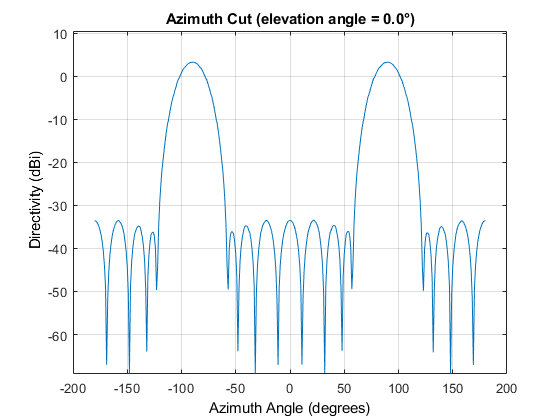
\includegraphics[width=\linewidth]{Pictures/overall_array/rectangular.png}
  \textit{\caption{Rectangular pattern}\label{fig:immagine3}}
\endminipage
\end{figure}

% Pattern on 45 
\newpage
Then we plotted the array pattern on $45 \degree$ with its Azimuth-cut and its rectangular pattern.

\begin{figure}[!htb]
\minipage{0.322\textwidth}
  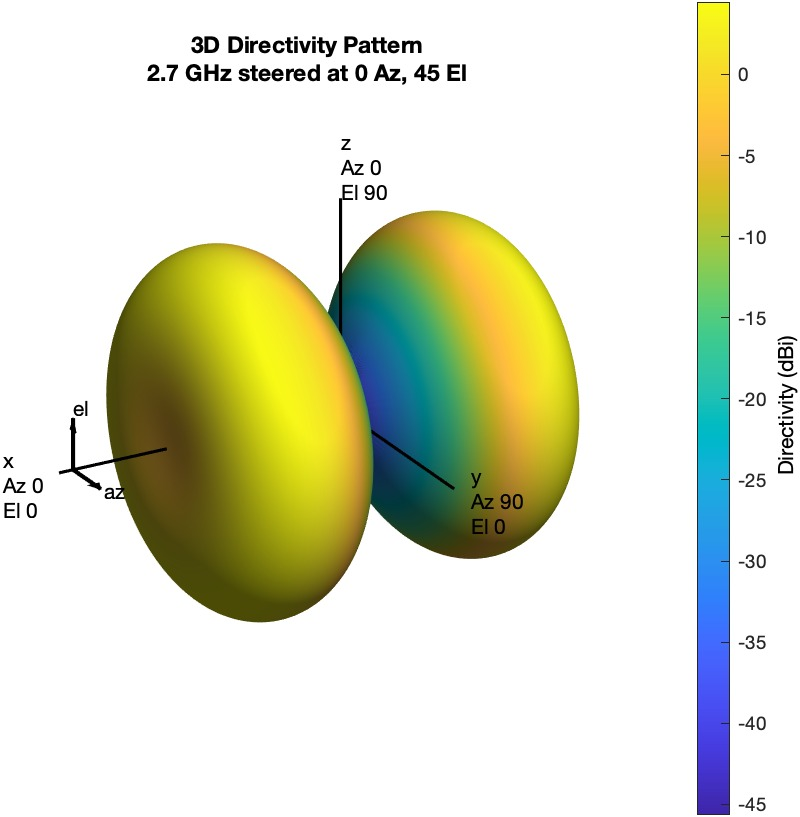
\includegraphics[width=\linewidth]{Pictures/overall_array/directivity_pattern_45deg.jpeg}
  \textit{\caption{Radiation pattern on $45\degree$}}
\endminipage\hfill
\minipage{0.322\textwidth}
  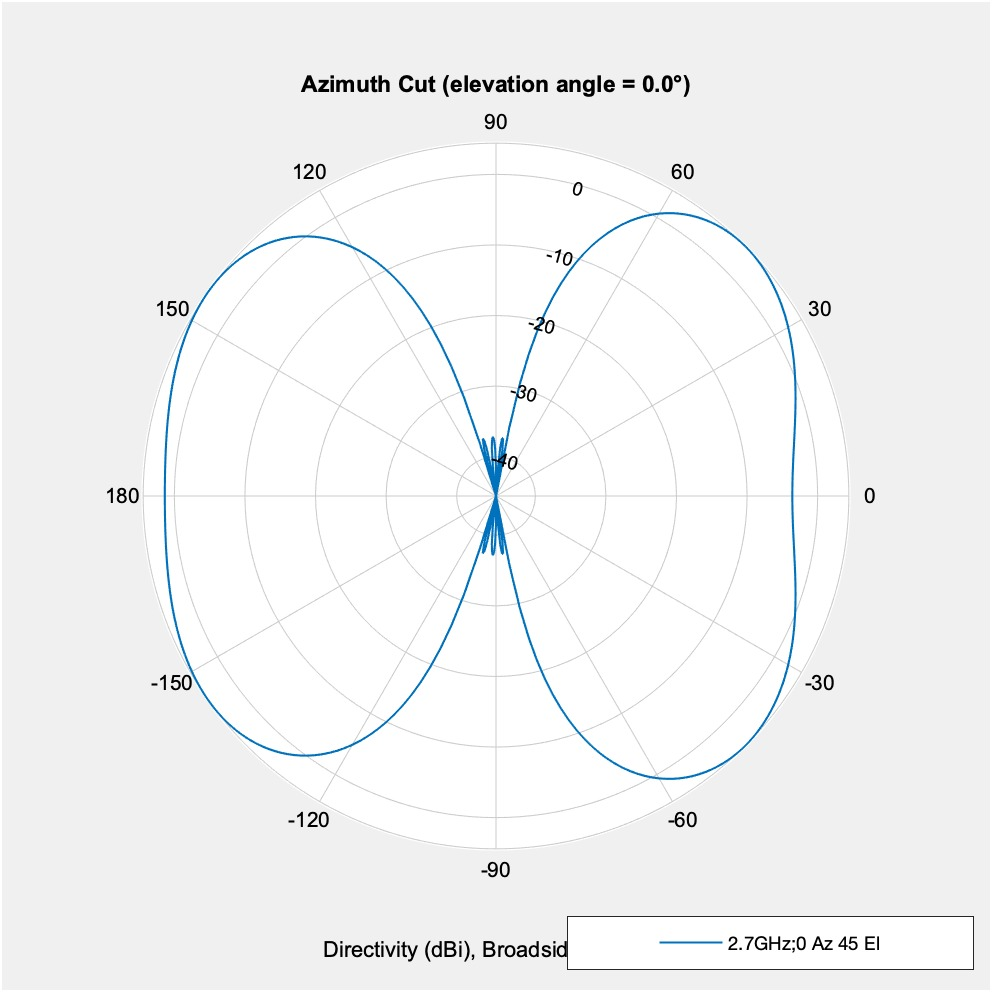
\includegraphics[width=\linewidth]{Pictures/overall_array/directivity_az_45deg.jpeg}
  \textit{\caption{Azimuth-cut on $45\degree$}}
\endminipage\hfill
\minipage{0.27\textwidth}
  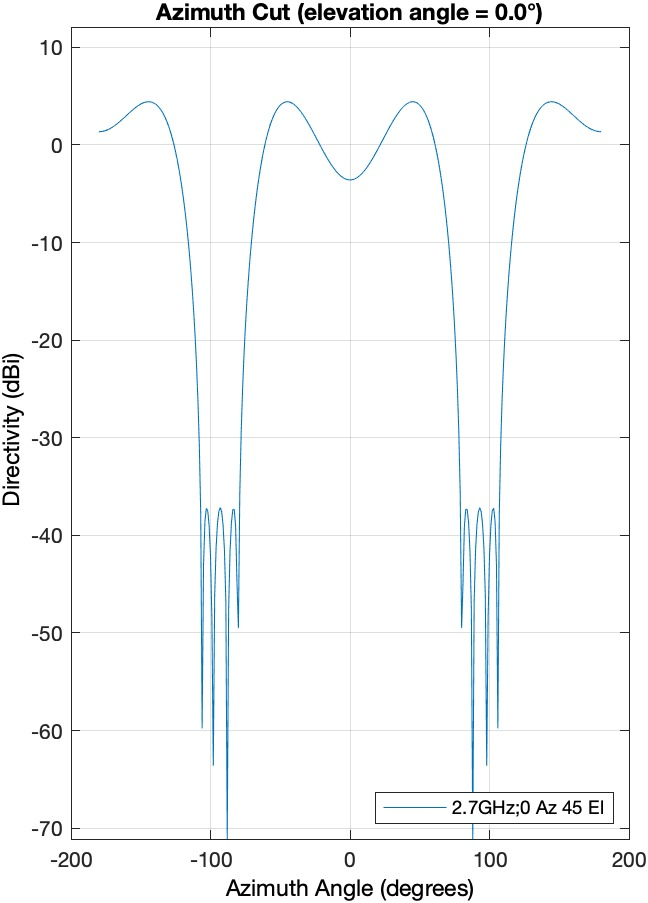
\includegraphics[width=\linewidth]{Pictures/overall_array/rectangular_45deg.jpeg}
  \textit{\caption{Rectangular pattern on $45\degree$}}
\endminipage
\end{figure}

\section{Total array gain by using pattern multiplication principle}
%2.	compute and plot the total array gain by using the pattern multiplication principle\newline
In order to compute the total array gain by using the pattern multiplication principle, we compute first the  gain of the array factor with isotropic elements. Considering the tapering efficiency $\eta_{T} = 78\%$ follow that:
\begin{equation}
G_{F} = \eta_{T} (2N+1) = 3.9, \quad
G_{Tot} = G_{element} G_{F}
\end{equation} in $~dBi$, is equal to $0.86 ~dBi$.\\
For what concern the $45\degree$ pointing is possible to compute the gain of array factor in that pointing direction by using the following formula:
\begin{equation}
G_{F}=\frac{\left|\sum_{n}\right( I_{n}\exp{(jn(u+u_{0}))}|^{2}}{\sum_{n}\left|I_{n}\right|^{2}}
\end{equation}

that considering the phase coefficient to achieve 45\degree, is equal to $3.165 ~(linear)$, converted to $dBi$ is equal to  $5~dBi$.
By multiply it for the gain of single element that is $G_{element}=-3.04 ~dBi$, we obtain the total gain $G_{Tot}$ = $1.96 ~dBi$.

\section{Total array gain with fullwave model}
%3.	compute and plot the total array gain by mean of a fullwave model of the array with Matlab MoM.\newline


\begin{figure} [h!]
\begin{minipage}[b]{7cm}
\centering
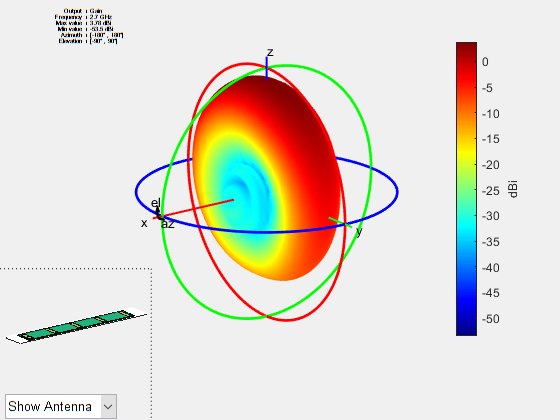
\includegraphics[width=6cm]{Pictures/overall_array/fullwave_arraycompelto.png}
\textit{\caption{3-D Broadside Gain pattern}}
\end{minipage}
\ \hspace{2mm} \hspace{3mm} \
\begin{minipage}[b]{7cm}
\centering
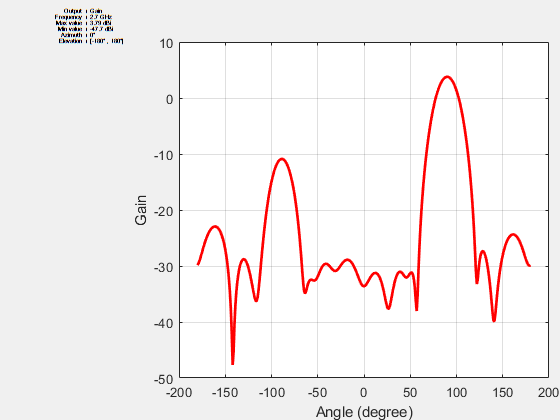
\includegraphics[width=6cm]{Pictures/overall_array/gain_ar_rectangular.png}
\textit{\caption{Rectangular Gain pattern}}
\end{minipage}
\end{figure}

The total gain obtained in the direction of maximum by the fullwave model is $3.79 ~dBi$, different of almost two dB from the one obtained with the multiplication principle due to the coupling antenna effects, neglected when multiplication principle is applied. Then we also computed and graphed the radiation pattern on $45 \degree$.

\begin{figure} [h!]
\begin{minipage}[b]{7cm}
\centering
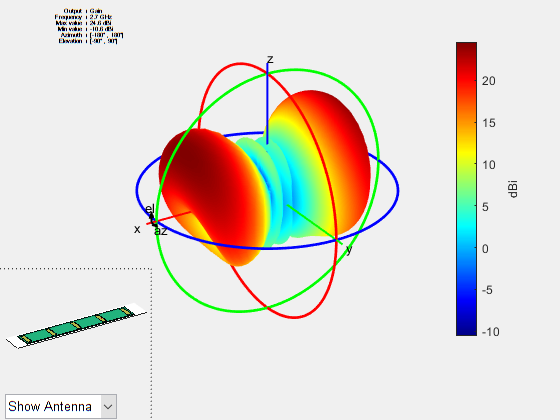
\includegraphics[width=6cm]{Pictures/overall_array/gain_fullwave_45deg_3d.png}
\textit{\caption{3-D Gain pattern on 45 $\degree$}}
\end{minipage}
\ \hspace{2mm} \hspace{3mm} \
\begin{minipage}[b]{7cm}
\centering
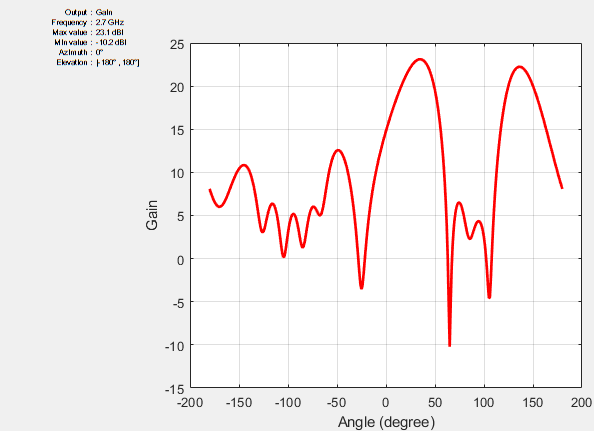
\includegraphics[width=6cm]{Pictures/overall_array/gain_45_fullwave.png}
\textit{\caption{Rectangular Gain on 45 $\degree$}}
\end{minipage}
\end{figure}

\newpage
\section{Near field analysis}
%4.	plot of the near field just over the array plane to analyze the fringing field from the edges and observe possible non-uniformity due to the inter-antenna coupling.\newline

As final step, we graphed the near field over the array plane to analyze the fringing field from the edges and observe possible non-uniformity due to the inter-antenna coupling.

\begin{figure} [h!]
\begin{minipage}[b]{7cm}
\centering
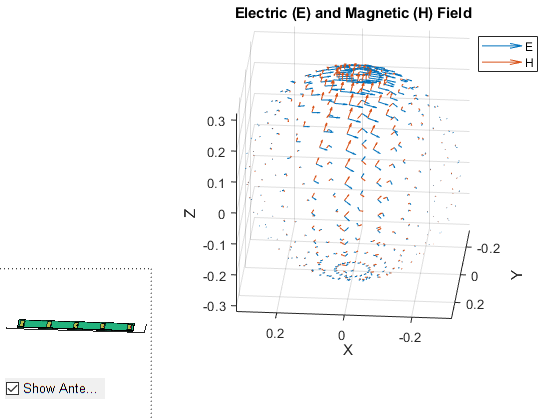
\includegraphics[width=8cm]{Pictures/overall_array/EHfield90.png}
\textit{\caption{E-H near field Broadside}}
\end{minipage}
\ \hspace{2mm} \hspace{3mm} \
\begin{minipage}[b]{7cm}
\centering
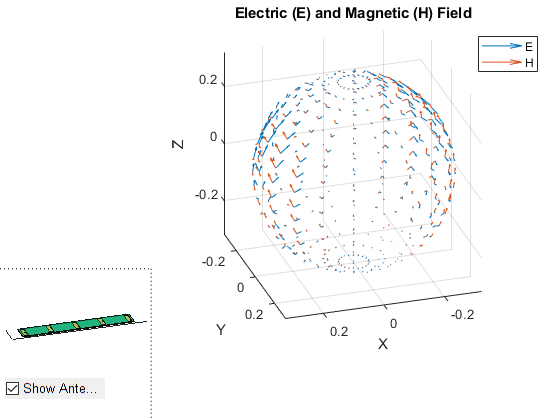
\includegraphics[width=8cm]{Pictures/overall_array/EHfields_45gradi.png}
\textit{\caption{E-H near field on $45 \degree$}}
\end{minipage}
\end{figure}

In the two images, fringing fields can be seen on the short sides of near field Broadside (figure 3.11) and partially on the long side of near field on $45 \degree$ (figure 3.12). Therefore, from the areas with different field strengths and the fact that the E-cut and H-cut planes cannot be distinguished, the non-uniformity due to coupling can be noted.

\end{document}